%-----------------------------------------------------------------------------
%
%               Template for sigplanconf LaTeX Class
%
% Name:         sigplanconf-template.tex
%
% Purpose:      A template for sigplanconf.cls, which is a LaTeX 2e class
%               file for SIGPLAN conference proceedings.
%
% Guide:        Refer to "Author's Guide to the ACM SIGPLAN Class,"
%               sigplanconf-guide.pdf
%
% Author:       Paul C. Anagnostopoulos
%               Windfall Software
%               978 371-2316
%               paul@windfall.com
%
% Created:      15 February 2005
%
%-----------------------------------------------------------------------------


\documentclass[preprint]{sigplanconf}

% The following \documentclass options may be useful:
%
% 10pt          To set in 10-point type instead of 9-point.
% 11pt          To set in 11-point type instead of 9-point.
% authoryear    To obtain author/year citation style instead of numeric.

\usepackage{amsfonts}
\usepackage{amsmath}
\usepackage{amsthm}
\usepackage{graphicx}
\usepackage{subfig}
\usepackage{epstopdf}
\usepackage{fancyvrb}
\usepackage{multicol}

\newtheorem{definition}{Definition}
\newtheorem{proposition}{Proposition}

\def\QED{\mbox{\rule[0pt]{1.5ex}{1.5ex}}}

\def\endproof{\hspace*{\fill}~\QED\par\endtrivlist}


\begin{document}

\conferenceinfo{PLDI '13}{June 16 -- 21, 2013, Seattle, Washington, USA.} 
\copyrightyear{2013} 
\copyrightdata{[to be supplied]} 

\titlebanner{banner above paper title}        % These are ignored unless
\preprintfooter{short description of paper}   % 'preprint' option specified.

\title{AutoSynch: An Automatic-Signal Monitor \\ Based on Predicate Tagging}
\subtitle{}

\authorinfo{Wei-Lun Hung\and Vijay K. Garg}
           {The University of Texas at Austin}
           {wlhung@utexas.edu, garg@ece.utexas.edu}

\maketitle

\begin{abstract}
For more than forty years, monitor has been used by the parallel programming 
community as the main mechanism for mutual exclusion and conditional 
synchronization. An 
automatic-signal monitor uses the $waituntil$ statement for conditional 
synchronization, while the explicit-signal monitor uses condition variables and 
$signal/wait$ statements. Despite the simplicity of the automatic-signal monitor, 
most of the modern programming languages support only the explicit-signal 
monitor but not the automatic-signal monitor because of the performance issues. 
In this paper, we argue that the automatic-signal monitor can be as efficient 
as explicit-signal monitor or even more efficient for some cases.

To satisfy the need for automatic-signal monitor, we propose a system called 
AutoSynch that allows gains in productivity of 
programmers as well as gain in performance. We introduce an operation called
$globalization$ that enables the predicate evaluation in
every thread. Based on this operation, AutoSynch provides $relay\ guarantee$
that some thread waiting for a condition has been met is always signaled; 
therefore, the $signalAll$ call is avoidable in AutoSynch. For efficiency in 
deciding which thread should be signaled, AutoSynch uses 
$predicate\ tagging$, in which tags are assigned to every predicate according
to its semantics. AutoSynch can find and signal an appropriate condition 
variable efficiently by examining the state of a monitor and tags. 

To evaluate the efficiency of AutoSynch, we implemented many different 
well-known synchronization problems such as the producers/consumers problem,
the readers/writers problems, and the dining philosophers problem. The results
suggest that AutoSynch is almost as efficient as the explicit-signal monitor
and even more efficient for some cases. 

\end{abstract}

\category{CR-number}{subcategory}{third-level}

\terms
Algorithms, Languages, Performance 

\keywords
automatic signal, concurrency, explicit signal, implicit signal, monitor, 
parallel


% code examples


\section{Introduction} \label{sec:intro}
%Developing efficient and robust concurrent programs within a limited time is 
%critical than ever. On the one hand, the multi-core processor, which allows 
%multiple threads to be executed at the same time, has become the mainstream of 
%computers; however, the power of multi-core processors is limited due to the 
%lack of concurrent applications. In order to compete with other rivals
%and to satisfy consumers' demands in the software industry, applications need to be
%developed in a shot period. The concurrent programming is 
%different from the traditional sequential programming. Multiple threads may 
%interact with each other and try to access the same source. Form the programmers' perspective, 
%it is much more difficult to correctly develop concurrent programs than sequential programs. 
%In addition, the debugging process is panic in concurrent programs due to the 
%thread scheduling. 

%The monitor \cite{hoa74, bh75a} is commonly used in the concurrent programming for 
%maintaining the mutual exclusion of shared resources and providing the 
%synchronization mechanism between threads. Buhr and Harji \cite{bh05} divided 
%monitors into two categories, the explicit-signal monitor and the 
%automatic-signal monitor. Buhr and Harji used the explicit-signal monitor to 
%simulate the automatic-signal monitor and pointed out that the automatic-signal 
%monitor is not as efficient as the explicit-signal monitor. However, the 
%automatic-signal is easy to be used and useful in concurrent programming,
%especially for prototyping. 

%Most programming languages, including the popular object-oriented language Java,
%only provide the explicit-signal monitor but not automatic-signal. This research 
%focuses on developing a framework supporting automatic-signal monitor without
%sacrificing efficiency in the modern programming language - Java. 

%our contribution


The multicore hardware is now ubiquitous. Even the cell phones have
multicore processors. Programming these multicore processors is
still a challenging task due to
bugs resulting from concurrency and synchronization.
Although there is widespread acknowledgement of difficulties 
in programming these systems, it is hard to believe that by and large the most 
prevalent methods of dealing with synchronization are based on ideas that were 
developed in early 70's \cite{dijk68, hoa74, bh75a}. For 
example, the most widely used threads package in C++ \cite{stro97}, 
pthreads \cite{bute97}, and the most widely used package in Java \cite{gjs00}, 
java.util.concurrent \cite{lea05}, are based
on the notion of monitors \cite{hoa74, bh75a}(or semaphores \cite{dijk68}) 
developed in 60's and 70's.
In this paper, we propose a new method called AutoSynch 
that allows gains in productivity of the programmer as well as gain in
performance of the system.

%\subsection{Why Is Automatic-Signal Monitor Needed?}
Both pthreads and Java require programmers to explicitly
signal threads that may be waiting on certain condition. The programmer
has to explicitly declare condition variables and then signal one
or all of the threads when the associated condition becomes true.
Using the wrong notification ($signal$ versus $signalAll$) is a frequent
source of bugs. In AutoSynch there is no notion of condition variables
and it is the responsibility of the system to signal appropriate threads.
This feature in AutoSynch significantly reduces the program size and complexity.
Note that the idea of automatic signaling has been proposed 
in the original paper by Hoare as \cite{hoa74}. Buhr and Harji use implicit
signal an alternative to automatic signaling \cite{bh05}. 
However, it is generally believed that automatic 
signaling is extremely inefficient compared to explicit signaling. 
For example, Buhr, Fortier, and Coffin claim that automatic monitors are 10-50 times
slower than explicit signals \cite{bfc95}. The reason for the slowdown is that
previous implementations of automatic monitor are based on the
evaluation of all conditions, whenever monitor is available. We show in this
paper that the widely held belief is wrong. 
%\subsection{AutoSynch Example}
%The concurrent programs are more difficult to be written and debugged than the 
%sequential programs. Although explicit-signal monitor already provides an 
%elegant mechanism for programmers to maintain mutual exclusion and synchronization 
%in concurrent programs; automatic-signal is more straightforward in both code
%reasoning and syntax. 

To make the automatic-signal mechanism available in Java, we proposes the 
framework of AutoSynch illustrated in Fig.~\ref{fig:fw}. 
The AutoSynch framework is composed of a 
preprocessor and a Java condition manager library. The preprocessor translates 
AutoSynch code into traditional Java code. Our automatic-signal mechanism and 
developed techniques were implemented in the Java library. Although this paper 
focuses on Java, our techniques are also applicable to other programming 
languages and models, such as pthread and C\# \cite{hwg03}.

%Fig.~\ref{fig:fw} illustrates the framework of AutoSynch, which makes 
%the automatic-signal available with the modern high-level language, Java. 
%The AutoSynch takes a Java-extension program providing the automatic-signal 
%mechanism through supporting the monitor class and the waituntil statement. The 
%AutoSynch preprocessor transfers an AutoSynch code into the tradition Java code 
%that can be compiled with AutoSynch library. The AutoSynch 
%Java library implements our automatic-signal monitor mechanism.  
%
\begin{figure}[ht!]
  \centering
  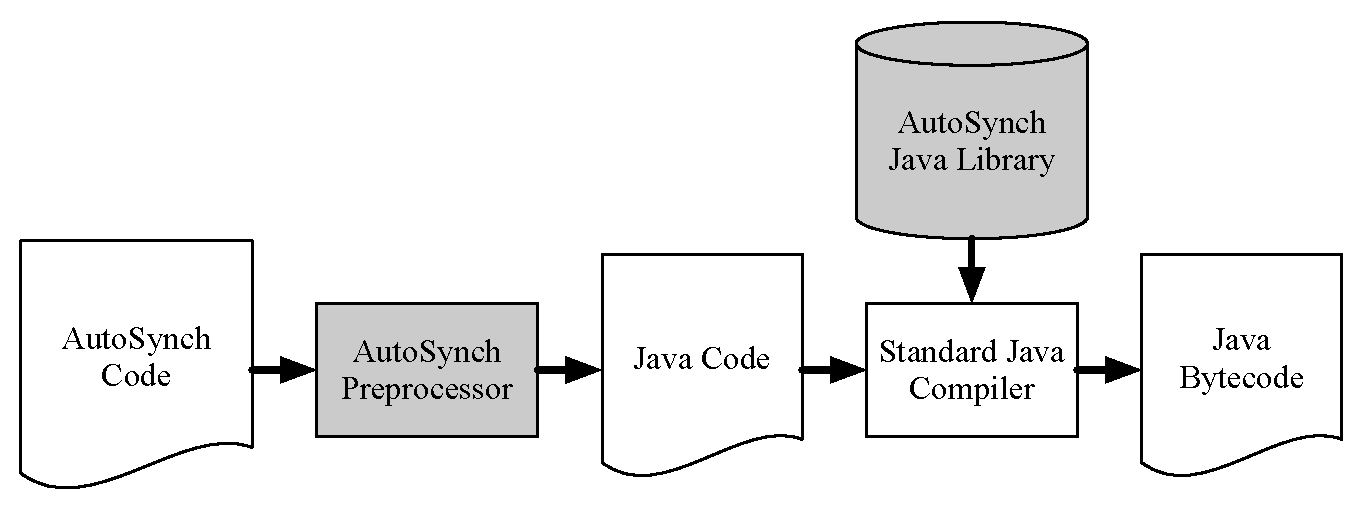
\includegraphics[width=80mm]{fig/flow.eps}
  \caption{The framework of AutoSynch}
  \label{fig:fw}
\end{figure}


AutoSynch extends Java with supporting the $AutoSynch$ class and the
$waituntil$ statement \cite{gm05}. In an $AutoSynch$ class, every member 
function can be executed by 
only one thread at any time; i.e., an $AutoSynch$ class provides  
mutual exclusion by default. The $AutoSynch$ is reserved as a modifier, 
indicating a $AutoSynch$ class. A $waituntil$ statement, appearing in 
only member functions of a $AutoSynch$ class, has a predicate as its parameter. 
When a thread is executing a $waituntil$ statement, it checks whether or not the 
predicate is true. The thread can continue to execute only when the predicate
is true. Otherwise, if the predicate is false, the executing thread must wait 
and release the privilege of the monitor control temporarily. 

Fig.~\ref{fig:bb_exp} shows an example demonstrating the difference between 
the Java implementation and the AutoSynch implementation for the 
bounded-buffer problem, also known as the producer-consumer problem. 
In the problem, two kinds of threads, producers and consumers, tries to obtain 
access to the shared resources. Producers put items 
into the buffer, while consumers take items out from the buffer. Every 
operation should be under mutual exclusion. Furthermore, a producer must wait  
when the buffer is full, while a consumer has to wait when the 
buffer is empty. The explicit-signal bounded buffer is written in Java. A 
lock variable and two condition variables are needed to maintain mutual exclusion 
and conditional synchronization. A thread needs to acquire the lock before entering member
functions. In addition, programmers need to explicitly associate conditional 
assertions with condition variables and call signal or await function manually.
On the contrary, 
the automatic-signal bounded buffer is written in our AutoSynch framework.
Programmers use $AutoSynch$ modifier to indicate the class is a monitor as line 
1. Besides, programmers use only $waituntil$ as in line 9 for conditional
synchronization. As can be expected, the automatic-signal monitor is
more straightforward and simpler than the explicit-signal monitor to
programmers. 
\begin{figure*}[ht!]
\begin{multicols}{2}
    \begin{Verbatim}[fontsize=\footnotesize,gobble=8,frame=topline,
            framesep=5mm,numbers=left,numbersep=2pt,
            label=\fbox{\small\emph{Explicit-Signal}}]
        class BoundedBuffer {
          Object[] items;  
          int putPtr, takePtr, count;
          Lock mutex = new ReentrantLock();
          Condition notFull = mutex.newCondition();
          Condition notEmpty = mutex.newCondition();
          public BoundedBuffer(int n) {
            items = new Object[n];
            putPtr = takePtr = count = 0;
          }
          public void put(Object x) {
            mutex.lock();
            while (count == items.length) {
              notFull.await();
            }
            items[putPtr++] = x;
            if (putPtr == items.length) {
              putPtr = 0;
            }
            ++count;
            notEmpty.signal();
            mutex.unlock();
          }
          public Object take() {
            mutex.lock();
            while (count == 0) {
              notEmpty.await();
            }
            int x = items[takePtr];
            if (takePtr == items.length) {
              takePtr = 0;
            }
            --count;
            notFull.signal();
            mutex.unlock();
            return x;
          }
        }
    \end{Verbatim}
    \begin{Verbatim}[fontsize=\footnotesize,gobble=8,frame=lines,framesep=5mm,
            numbers=left,numbersep=2pt,
            label=\fbox{\small\emph{Automatic-Signal}}]
        AutoSynch class BoundedBuffer { 
          Object[] items; 
          int putPtr, takePtr, count; 
          public BoundedBuffer(int n) {
            items = new Object[n];
            putPtr = takePtr = count = 0;
          }
          public void put(Object x) { 
            waituntil(count < items.length); 
            items[putPtr++] = x; 
            if (putPtr == items.length) { 
              putPtr = 0; 
            } 
            ++count; 
          } 
          public Object take() { 
            waituntil(count > 0); 
            Object x = items[takePtr++]; 
            if (takePtr == items.length) { 
              takePtr = 0; 
            }
            --count;
            return x;
          }
        }
    \end{Verbatim}
\end{multicols}
  \caption{Bounded-buffer example}
  \label{fig:bb_exp}
\end{figure*}

%\subsection{Design Principles}
In this paper we argue that automatic signaling is generally as fast as explicit 
and even faster for some examples. In Section \ref{sec:sigAll}, we give reasons
for the efficiency in automatic signaling. In short, the explicit signaling has 
to resort to $signalAll$ in some examples; however, our automatic signaling never 
uses $signalAll$. We have built AutoSynch that is almost always as 
fast as explicit and considerably faster for synchronization problems with 
$signalAll$. The design principles underlying AutoSynch are as follows.

\begin{description}
    \item{\bf Reduce context switches.} Context switch requires a certain 
        amount of time to save and load registers and update various tables and
        lists. Reducing unnecessary context switches boosts the performance.
        A $signalAll$ call introduces unnecessary context switches; therefore,
        $signalAll$ calls are forbidden in AutoSynch. 
    \item {\bf Reduce the number of unnecessary predicate evaluation.} In the 
        automatic-signal mechanism, automatically signaling a thread is the 
        responsibility of our system. The number of predicate evaluations is 
        crucial for efficiency in deciding which thread should be signaled. 
        Lower the number, better the performance.
\end{description}


%\subsection{Contributions}
The starting point in the design of AutoSynch is how to evaluate predicates of
$waituntil$ statements. Any thread that can access a monitor should be able
to check all predicates of $waituntil$ statements of the monitor. Therefore, a 
thread can decide which thread should be signaled according to the results of
predicate evaluations before the thread waits or exits the monitor. We 
investigated globalization operation to enable predicate evaluations in any 
thread. Based on this operation, our framework can provide relay guarantee and 
predicate tagging. 

To avoid using $signalAll$ call, AutoSynch 
provides relay guarantee, which ensures that some thread waiting for a
condition has met is always signaled. With this guarantee, the $signalAll$ call 
is unnecessary in our automatic-signal mechanism. Therefore, AutoSynch reduces 
the number of context switches by avoiding $signalAll$ calls. 

To accelerate the process in deciding which thread to be signaled, predicate 
tags are used for classifying predicates. Tags are assigned to every predicate
according to the semantics of the predicate. In deciding which thread should be 
signaled, we identify tags that are most likely to be true after examining the 
current state of a monitor. Then we only need to check the predicates with 
those tags. 

Our experimental results indicate that AutoSynch can significantly improve
performance compared to other automatic-signal mechanisms \cite{bh05}. It is
the generally believed that the automatic-signal mechanism is 10-50 times
slower than the explicit-signal mechanism \cite{bfc95}; however, AutoSynch is 
only 2.33 times slower than the explicit-signal mechanism in the worst 
case of our experiment results. Furthermore, AutoSynch is 288 
times faster than the explicit-signal mechanism in the case that rely on 
$signalAll$ calls. Besides, the experimental results also shows that AutoSynch 
is scalable; the performance of AutoSynch is stable even if the number of 
threads increases. 


The relationship between the automatic-signal and explicit-signal monitor can be 
depicted by analogy with the relationship between the garbage collection and 
manual memory management. Although garbage collection leads to decreased
performance because of the overhead in deciding which memory to free; programmers 
avoid manual memory deallocation. As a consequence, memory leaks and certain 
bugs, such as dangling pointer bugs and double free bugs, are reduced and 
eradicated. Similarly, automatic-signal mechanism consumes computing resources 
in deciding which thread to be signaled; programmers avoid explicitly invoking 
$signal$ calls. As a result, some bugs, such as using wrong notification and
signaling a wrong condition variable, are diminished and eliminated. 

Our main contributions are as follows.
\begin{enumerate} 
    \item We present the globalization, relay guarantee, and predicate tagging
        techniques that make automatic-signaling efficient. Experimental 
        evaluation of AutoSynch shows significant improvements in performance 
        and scalability with predicate tagging and relay guarantee. 
    \item We propose the design and implementation of the AutoSynch framework,
        which supports concurrent programs with automatic-signal mechanism.
    \item We show that the $signalAll$ call may introduce unnecessary context
        switches that decrease the performance. 
    \item We give experimental evidence indicating that AutoSynch's automatic-signal
        mechanism is almost as efficient as explicit-signal mechanism or even 
        more efficient with much simpler code.
\end{enumerate} 

%In this project, we are developing multiple such features. 
%Our second goal for SuperSynch is that the performance of the system
%with SuperSynch is at least as good as that for traditional systems.
%Continuing with the previous example of signaling threads,
%it is easy to develop automatic signaling mechanisms if performance
%is not an issue. For example, one could evaluate conditions for all
%threads. However, such a system would be significantly slower
%than explicit signaling systems for most programs. In this project
%we are developing techniques that usually result in programs
%with automatic signaling that are faster than the programs
%with explicit signaling. Thus, we get simpler programs with 
%faster performance. 

%Another aspect we are investigating in SuperSunch is the 
%idea of abortable monitor methods. The abortable methods 
%will support two widely used and familiar methods of programming
%(but not supported either by pthreads or Java). The 
%first notion is that of abortable transactions used in databases
%for decades. Although the concept has now entered in concurrent programming world 
%via transactional memories
%\section{Design of AutoSynch} \label{sec:fw}

This paper is organized as follows. Section \ref{sec:bg} gives the background
of montior. 
Section \ref{sec:sigAll} explains why $signalAll$ is required for
explicit-signal monitor but not automatic-signal monitor. The concepts of 
AutoSynch are presented in Section \ref{sec:concept} and the practical 
implementation details are discussed in Section  \ref{sec:imp}. The proposed 
methods are then evaluated with experiments in Section \ref{sec:eval}.  
Section \ref{sec:dis} and Section \ref{sec:conclu} give the discussions and the 
concluding remarks.

\section{Background: monitor} \label{sec:bg} 
%\subsection{Monitor}
Monitor is an abstract object or module containing shared data to be used safely
by multiple member functions and threads in concurrent programming. Monitor can
be defined by two characteristics, mutual exclusion and conditional 
synchronization. Mutual exclusion guarantees that at most one thread can 
execute any member function of a monitor at any time.  In general, threads need to acquire the lock of a monitor 
to acquire the privilege for accessing the monitor. Conditional synchronization 
maintains the executing order between threads. Threads may wait for some 
condition to be met and release the monitor lock temporarily. After the 
condition has been met, threads then re-acquire the lock and continue to 
execute. According to Buhr and Harji \cite{bh05}, monitors can be divided into 
two categories according to the different implementations of conditional 
synchronization. 
\begin{description}
    \item{\bf Explicit-signal monitor} In this type of monitor, condition
    variables, signal and await functions are used for synchronization. 
    Programmers need to associate assertions with condition variables manually.
    This mechanism involves two threads. One thread checks if some
    assertion is met or not, and then explicitly waits on some condition variable 
    if the assertion is not met. When another thread detects that the state has 
    changed and the assertion is met, it explicitly signals the 
    appropriate condition variable.
    \item{\bf Automatic-signal (implicit-signal) monitor} This kind of monitor 
    uses $waituntil$
    statements, such as line 9 in automatic-signal program in
    Fig.~\ref{fig:bb_exp}, instead of condition variables for
    synchronization. Programmers do not need to associate assertions with
    variables, but use $waituntil$ statements directly. In
    monitor, a thread will wait if the condition of a $waituntil$
    statement is false, and execute the remaining tasks after the condition 
    becomes true. The responsibility of signaling a waiting thread is that of 
    the system rather than of the programmers. 
\end{description}

Obviously, the explicit-signal is more complex than the automatic-signal monitor 
for programmers. The explicit-signal requires that programmers
have to write their conditional synchronization manually, which increases the 
chance of writing incorrect code. It is generally believed that that 
explicit-signal 
monitor is much faster than the automatic-signal monitor. In this paper, we 
argue that the automatic-signal monitor could be as efficient as the
explicit-signal or ever faster in some cases. 

\section{Why is signalAll required in the explicit-signal mechanism?} 
\label{sec:sigAll}
The $signalAll$ call is essential in explicit-signal mechanism when programmers
do not know which thread should be signaled. Fig.~\ref{fig:sigAll_exp}
illustrates an example. This example is also a bounded-buffer problem but 
different from Fig.~\ref{fig:bb_exp}. In this example, both $put$ and $take$
function have a parameter, $num$, indicating how many items are put or taken. 
Every producer and consumer can put and take a different number of items
every time.  Furthermore, a producer must wait if there is no space to put
$num$ items, while a consumer has to hold when the buffer has insufficient items.
Note that, since the parameter $num$ may be different every time, every 
consumer and producer may wait on a different condition to be met; programmers 
do not know which producer or consumer should be signaled at runtime. 
Therefore, the $signalAll$ calls should be used instead of $signal$ calls in
line 23 and 39.
Although programmers can avoid using $signalAll$ calls by writing
complicated code that associates different conditions to different condition 
variables; the complicated code makes the maintenance of the program
unsustainable. 

The $signalAll$ call is bad; it may decreases the performance because 
it introduces redundant context switches, requiring a certain 
computing time to save and load registers and update various tables and lists.
Furthermore, $signalAll$ calls cannot increase parallelism because threads
are forbidden to access a monitor simultaneously. Although multiple threads are
signaled at a time, only one thread is able to acquire the monitor. Other 
threads may need to go back to waiting state since another thread may change 
the status of the monitor. For example, in Fig.~\ref{fig:sigAll_exp}, the 
buffer has 64 items after a producer finishes a put call. The producer calls 
$insufficientItem.signalAll()$ in line 23 before completing the call. 10  
waiting consumers are signaled; each of them is waiting to take $48$ items.
Suppose the consumer $C_1$ re-acquires the lock first and takes $48$ items. The
remaining items, $16$, are insufficient for the other threads; they
make context switches, re-evaluate their predicates, and go back to waiting 
state. Theses context switches are redundant since the 9 threads do not 
make any progress but only go back to waiting. 
Therefore, if we avoid using the $signalAll$ call and only signal a thread that 
is most likely to make progress, the unnecessary context switches can be
reduced.

\begin{figure}[ht!]
    \begin{Verbatim}[fontsize=\footnotesize,gobble=8,frame=lines,
            framesep=5mm,numbers=left,numbersep=2pt,
            label=\fbox{\small\emph{Explicit-Signal}}]
        class BoundedBuffer {
          Object[] items;  
          int putPtr, takePtr, count;
          Lock mutex = new ReentrantLock();
          Condition insufficientSpace = mutex.newCondition();
          Condition insufficientItem = mutex.newCondition();
          public BoundedBuffer(int n) {
            items = new Object[n];
            putPtr = takePtr = count = 0;
          }
          public void put(int num) {
            mutex.lock();
            while (num + count > items.length) {
              insufficientSpace.await();
            }
            for (int i = 0; i < num; ++i) {
              items[putPtr++] = new Object();
              if (putPtr == items.length) {
                putPtr = 0;
              }
            }
            count += num;
            insufficientItem.signalAll();
            mutex.unlock();
          }
          public Object[] take(int num) {
            mutex.lock();
            while (count < num) {
              insufficientItem.await();
            }
            Object[] ret = new Object[n];
            for (int i = 0; i < num; ++i) {
              ret[i] = items[takePtr++];
              if (takePtr == items.length) {
                takePtr = 0;
              }
            }
            count -= num;
            insufficientSpace.signalAll();
            mutex.unlock();
            return ret;
          }
        }
    \end{Verbatim}
    \caption{Bounded-buffer* example}
    \label{fig:sigAll_exp}
\end{figure}


\section{AutoSynch concepts} \label{sec:concept}


\subsection{Predicate evaluation}
%In order to allow any thread that can access a monitor to evaluation all
%predicates of waiting threads, an operation called globalization is defined as 
%replacing all local variables of
%a predicate by its values at the time. The globalization converts a local 
%predicate into a global predicate since all the local variables have been 
%replaced. The globalization has an important characteristic that allows a
%local predicate to be evaluated by any other thread safely after the original
%thread waits. The reason is that no other thread can access to the local variables of a member 
%function in which a particular thread is executing; therefore values of local variables 
%cannot be changed by other threads after a particular thread is waiting. 
%All other threads can check the globalized predicate safely. 
%\subsection{Predicate}
In AutoSynch, it is the responsibility of the system to signal appropriate 
threads automatically. The predicate evaluation is crucial in deciding which
thread should be signaled. We will discuss how to preform predicate evaluations
of $waituntil$ statements. 

A predicate $P(\vec{x}): X \rightarrow \mathbb{B}$ is a Boolean condition, 
where $X$ is the space spanned by the variables $\vec{x}=(x_1, \dots, x_n)$. 
A variable of a monitor object is a shared variable if it is accessible to every 
threads that are accessing the monitor. The set of shared variables is denoted by 
$S$. The set of local variables, denoted by $L$, is 
accessible only by a thread calling a function in which the variables are declared. 

Predicates can be used to describe the properties of conditions. In this paper,
every condition of $waituntil$ statement is represented by a predicate. We say
a condition has met if its representing predicate is true; otherwise, the
predicate is false. 
Furthermore, we assume that every predicate, $P = \vee_{i=1}^nc_i$, is in 
disjunctive normal form (DNF), where $c_i$ is defined as the conjunction of a 
set of atomic Boolean expressions. For example, a predicate $(x = 1) \wedge 
(y = 6) \vee (z \ne 8)$ is DNF, where $c_1 = (x = 1) \wedge (y = 6)$ and $c_2 = 
(z \ne 8)$. Note that, every Boolean formulas can be converted into DNF using 
De Morgan's laws and distributive law. 

Predicates can be divided into two categories based on the type of their 
variables \cite{bh05}.
\begin{definition}[Shared and general predicate]
    Consider a predicate $P(\vec{x}): X \rightarrow \mathbb{B}$. If $X 
    \subseteq S$, $P$ 
    is a shared predicate. Otherwise, if $X \not\subseteq S$, $P$ 
    is a general predicate. 
\end{definition}

The automatic-signal monitor has an efficient implementation \cite{kes77} by 
limiting the predicate of a $waituntil$ to a shared predicate; however, 
we do not limit the predicate of a $waituntil$ statement to a shared
predicate. The reason is that this limitation will lead AutoSynch to be less
attractive and practical since conditions including local variables cannot be 
represented in AutoSynch.

Evaluating a general predicate in all threads is unattainable 
because the accessibility of the local variables in the predicate is limited 
to the thread declaring them. To evaluate a general predicate in all 
threads, we treat local variables as constant values at runtime and define 
globalization as follows. 
\begin{definition}[Globalization]
    Given a general predicate $P(\vec{x}, \vec{y}): X \times Y \rightarrow 
    \mathbb{B}$, where $X \subseteq S$ and $Y \subseteq L$. The globalization 
    of $P$ at runtime $t$ is the new shared predicate
    \[
    G_t(\vec{x}) = P(\vec{x}, \vec{y_t}),
    \]
    where $\vec{y_t}$ is the values of $\vec{y}$ at runtime $t$.
\end{definition}

The globalization can be applied to any general predicate; a shared 
predicate is derived form the globalization. For example, consider a 
general predicate $(x = v)$, where $x$ is a shared variable and $v$ is a local
variable. Suppose at runtime $t$, the value of $v$ is $6$; i.e., $v_t=6$. We
apply the globalization at $t$ and derive a shared predicate $(x = 6)$. 

The following proposition shows that the general predicate evaluation of
$waituntil$ statement in all thread can be achieved through the globalization. 
\begin{proposition} \label{pro:glob}
    Consider a general predicate $P(\vec{x}, \vec{y})$ in a $waituntil$ 
    statement. $P(\vec{x}, \vec{y})$ and its globalization 
    $P(\vec{x}, \vec{y_t})$ are semantically equivalent during the $waituntil$ 
    period, where $t$ is the time instant immediately before invoking the 
    $waituntil$ statement.  
\end{proposition}
\begin{proof}
    Only the thread invoking the $waituntil$ statement is able to access the
    local variables of the predicate; all other threads are unable to change
    the values of those local variables. Therefore, the value of $\vec{y}$
    cannot be changed 
    during the $waituntil$ period. Since $\vec{y_t}$ is the value of $\vec{y}$
    immediately before invoking the $waituntil$ statement, $P(\vec{x}, \vec{y})$
    and $P(\vec{x}, \vec{y_t})$ are semantic equivalent during the $waituntil$
    period. 
\end{proof}

Proposition \ref{pro:glob} enables the general predicate evaluation of
$waituntil$ statement in all threads. 
Given a general predicate in a $waituntil$ statement, in the sequel we substitute
all the local variables with their values immediately before invoking the
statement. The predicate can be evaluated in all other threads during the
$waituntil$ period. 

\subsection{Relay guarantee}
As mentioned in Section ~\ref{sec:sigAll}, $signalAll$ calls are unavoidable in
the explicit-signal mechanism sometimes; however, $signalAll$ calls may decrease
performance by introducing redundant context switches. 
In
AutoSynch, $signalAll$ calls are avoided by providing the following guarantee. 
%should be reduced. Before a waiting thread is signaled, the 
%predicate of the waiting thread is ensured to be true. In addition, at most 
%one waiting thread is signaled at any time. The reason is that threads are 
%forbidden to access a monitor simultaneously. Signaling multiple threads does 
%not increase parallelism but redundant context switches. 

\begin{definition}[Relay guarantee]
    Some thread waiting for a condition has met is eventually signaled; i.e., 
    suppose $W_T$ represents the set of waiting threads that their conditions 
    has become true, then
    \[
        W_T \ne \phi \Rightarrow \exists T \in W_T\ s.t.\ \Diamond T\ 
        is\ signaled.  
    \]
    
\end{definition}
\begin{proposition} \label{pro:one}
    Relay guarantee can be provided by the following procedure. When a thread 
    exits a monitor or goes into waiting state, it checks whether or not there 
    is some thread waiting on a condition that has been met. If
    at least one such waiting thread exists, the thread is signaled.
\end{proposition}
\begin{proof}
    Suppose not. All threads waiting for conditions have met are blocked and 
    no other thread can signal them. Consider a condition $P$ that has been 
    true. Since some thread goes into waiting state with $P$, $P$ is false
    initially. Some other threads must enter the monitor and change the status 
    of the monitor to make $P$ true. Suppose thread $T$ is the last thread 
    active in the monitor. According to the procedure, $T$ must signal one 
    thread waiting on $P$ or another thread waiting on another predicate that
    has been true before leaving or going into waiting state. It contradicts
    the assumption that all threads waiting for conditions have met are
    blocked and no other thread can signal them.   
 \end{proof}

The concept behind relay guarantee is that, the privilege of a monitor control
is transmitted from one thread to another thread waiting for a condition that 
has been met.
Relay guarantee never introduces deadlock; consequently, {\it signalAll} calls
are avoidable by providing relay guarantee. 
Proposition \ref{pro:one} lays the theoretical foundation that the relay
guarantee can be provided in our automatic-signaling mechanism. 
The remaining problem is how to find a thread waiting for a condition that has 
been met efficiently. 

\subsection{Predicate tag} 
In order to find an appropriate thread waiting for a predicate that has been
true efficiently, every predicate acquires different tags according to its 
semantics. Those tags depict the properties of a predicate; therefore, tags
help us prune predicates that are unable to be true through examining the state 
of a monitor. Before going through the details, two particular types of 
predicates are defined as follows according to their semantics. 
\begin{definition}[Local and general expression]
    Consider an expression $E(\vec{x}): X \rightarrow \mathbb{D}$, where
    $\mathbb{D}$ represents one of the primitive data types in Java. If $X
    \subseteq L$, $E$ is a local expression. Otherwise, if $X \not\subseteq L$,
    $E$ is a general expression.  
\end{definition}

\begin{definition}[Equivalence predicate]
    A predicate $P: (GE = LE)$ is an equivalence predicate, where $GE$ is a
    general expression, and $LE$ is a local expression.
\end{definition}
%\begin{definition}
%    A predicate $P: (v \neq c)$ is a non-equivalence predicate, where $v$ is the
%    pivot variable and $v \in S$, and either $c \in L$ or $c$ is a constant 
%    value.
%\end{definition}
\begin{definition}[Threshold predicate]
   A predicate $P: (GE\ \boldsymbol{op}\ LE)$ is a threshold predicate, where 
   $\boldsymbol{op}
    \in \{<,\ \le,\ >,\ \ge\}$, $GE$ is a general expression, and $LE$ is a
    local expression.
\end{definition}
Note that, many variables can be moved from one side to another side. For
example, the variable $a$ and $b$ in $x = (y - b) / a$ can be moved as 
$ax + b = y$. These two types of predicates can represent a wide range of
conditions in synchronization problems. 

The $globalization$ operation can also be applied to any general and local 
expression. Note that, applying the $globalization$ to a local expression
derives a constant value. For example, consider a local expression 
$E = a \times b + c$, $a = 2$, $b = 4$, and $c = 8$ at time $t$, $E$ is $16$
after applying the $globalization$ at time $t$. 

In general, tags are assigned to predicates according to their types. In 
AutoSynch, there are three types of tags, $Equivalence$, $Threshold$, and 
$None$. The formal definition of the tag is as follows. 
\begin{definition}
   A tag is a four-tuple $(M,\ expr,\ key,\ op)$, where  
   \begin{itemize}
      \item $M \in \{Equivalence,\ Threshold,\ None\}$;
      \item $expr$ is a general expression after applying globalization if 
          $M \in \{Equivalence,\ Threshold\}$; otherwise, $expr= \perp$;
      \item $key$ is the value of a local expression after applying
          globalization if $M \in \{Equivalence,\ Threshold\}$; otherwise, 
          $key= \perp$;
      \item $op \in \{<,\ \le,\ >,\ \ge\}$ if $M = Threshold$; otherwise, 
         $op = \perp$.
   \end{itemize}
\end{definition}
Every $Equivalence$ or $Threshold$ tag represents a equivalence predicate or 
threshold predicate respectively. For example, the tag 
$(Threshold,\ x + 8,\ 11,\ >)$ represents the predicate $x + 8 > 11$. 
We say a tag is true if the predicate represented by the tag is true; 
otherwise, we say the tag is false. 
\subsubsection{Predicate tagging}
Tags are given to every predicate by the algorithm shown in
Fig.~\ref{fig:tagging}. A tag is assigned to every conjunction. The tags of 
conjunctions of a predicate constitute the set of tags of the predicate. 
When assigning a tag to a conjunction, the equivalence tag has the highest 
priority than others. The reason is that an equivalence predicate is more
difficult to be true than other kinds of predicates since it is true only when 
its general expression equals a specific value. 
For example, consider an equivalence 
predicate $x = 8$ and a threshold predicate $x > 3$. $x = 8$ is true only when 
the value of $x$ is $8$. On the contrary, $x > 3$ is true for every value of 
$x$ is greater than $3$. Therefore, the $Equivalence$ tags can help us to prune
predicates that are unable to be true more efficiently than other kinds of
tags. Thus, we say $Equivalence$ predicates are more dominate than other
predicates in pruning predicates.  
If a conjunction does not 
include any equivalence predicate, then we check whether or not it 
includes any threshold predicate. If yes, then a $Threshold$ tag is assigned 
to the conjunction; otherwise, the conjunction has a $None$ tag. 

\begin{figure}[ht!]
    \begin{Verbatim}[fontsize=\footnotesize,gobble=8,frame=lines,
            framesep=3mm]
         tags = empty
         foreach conjunction c 
           if c contains an equivalence predicate ge=le
             tag t = (Equivalence, globalization(ge), 
                 globalization(le), null)
             add t to tags
           else if c contains a threshold predicate ge op le
             tag t = (Threshold, globalization(ge), 
                 globalization(le), op)
             add t to tags
           else 
             add (None, null, null, null) to tags
         return tags
    \end{Verbatim}
  \caption{Predicate Tagging}
  \label{fig:tagging}
\end{figure}
Creating all tags for a conjunction is unnecessary. If a conjunction includes 
multiple equivalence predicates or threshold predicates, only one arbitrary 
$Equivalence$ tag or $Threshold$ tag is assigned to the conjunction. 
If there are a large number of tags, then the performance may decrease
because of the cost of maintaining tags. As a result, we assign only one tag to
every conjunction. Furthermore, the motivation behind the predicate tag is to 
accelerate the searching process by pruning predicates that are unable to be
true but not exhaustive search for each tag.  Assigning multiple tags to a 
conjunction cannot accelerate the searching process. For example, consider a 
conjunction $(x = 8) \wedge (y = 9)$. If only a tag 
$(Equivalence,\ x,\ 8,\ null)$
is assigned to the conjunction, we check the predicate when the tag is
true. Adding another tag $(Equivalence,\ y,\ 9,\ null)$ cannot accelerate the
searching process since we need to check both tags. Hence, we create only one 
tag for each conjunction.
 


\subsubsection{Tag signaling}
Signaling mechanism is based on tags in AutoSynch. 
Since the equivalence tag is more dominate than the threshold tag, the
predicates with equivalence are checked prior to the predicates with other 
tags. If no predicate that is true can be found after checking $Equivalence$ 
tags and $Threshold$ tags, our algorithm does the exhaustive search for the 
predicates with $None$ tags. 

\paragraph{Equivalence tag signaling}
Observes that, an equivalence predicate becomes true only when its general
expression equals the specific value of its local expression after applying
$globalization$. For distinct equivalence tags related to a same general 
expression, at most one tag can be true at a time because the value of its
local expression is deterministic and unique at any time. By 
observing the value of the its local expression, the appropriate tag can be 
identified. For example, there are three $Equivalence$ tags for
predicates $x = 3$, $x = 6$, and $x = 8$. We examine $x$ and figure out that
its value is $8$. Then we know that only $x = 8$ is true. Based on this 
observation, for each unique general expression of an equivalence tag, we 
create a hash table, where the value of the local expression is used as the 
key. By using this 
hash table and evaluating the general predicate at runtime, we can find a
tag that is true in $O(1)$ time if there is any. Then we check the predicates 
with the tag. 

%Monotonic predicate evaluations can be optimized by the following observation. 
%\subsubsection{Non-Equivalence Predicate Signaling}
%Observing that, the value of a variable is deterministic and unique at any 
%time. Two distinct non-equivalence predicates with a same pivot variable cannot
%be false simultaneously. For example, at least one of $x \ne 8$ and $x \ne 5$
%is true. Non-equivalence predicates with a same pivot variable are stored in
%a linked list. By checking the first two predicates of the 
%linked list, at least one predicate is true. 

\paragraph{Threshold tag signaling}
For threshold tag, we consider the following situation. Suppose there are two 
predicates, $x > 5$ and $x > 3$, we know that if $x > 3$ is false, and then 
$x > 5$ cannot be true. That is, we only need to check the predicate with the 
smallest local expression value for $>$ and $\ge$ operations. Furthermore, 
consider the predicates with the same local expression value but different 
operations, $x > 3$ and $x \ge 3$. The predicate $x > 3$ cannot be true when 
$x \ge 3$ is false; i.e., we only need to check the predicate $x \ge 3$. We use
a min-heap data structure for storing the threshold tags related to a same 
general expression with $\boldsymbol{op} \in \{>, \ge\}$. If two predicates 
have a same local expression value but different operations, then the predicate 
with $\boldsymbol{op}=\ge$ is considered that it has the smaller value than the 
predicate with $\boldsymbol{op}=>$ in the min-heap.
Similarly, the max-heap can be used for threshold tags with $\boldsymbol{op}
\in \{<, \le\}$. Note that, if two predicates have a same local expression 
value but different operations, then the predicate 
with $\boldsymbol{op}=\le$ is considered that it has the larger value than the 
predicate with $\boldsymbol{op}= <$ in the max-heap.

%Def.~\ref{def:th_order} gives the formal definition of the 
%order for threshold tags. 

%\begin{definition} \label{def:th_order}
%    An ordering $\prec$ is defined as follows
%\[
%   (c_1, \boldsymbol{op}_1) \prec (c_2, \boldsymbol{op}_2)
%\]
%if and only if $c_1 < c_2$ or $c_1 = c_2$ and $(\boldsymbol{op}_1,
%\boldsymbol{op}_2)  = (\ge, >)$ or $(\boldsymbol{op}_1, \boldsymbol{op}_2) =
%(<, \le)$. 
%\end{definition}

The signaling mechanism for threshold tag is shown if Fig.~\ref{fig:th_sig}. In
general, the tag in the root of a heap is checked. If the tag is false, all the
descendant nodes are also false. Otherwise, all predicates with the tag
need to be checked for finding a true predicate. To maintain the correctness, 
if no predicate is true, the tag is removed from the heap temporarily. Then the
tag in the new root is checked again until a true predicate is found or a
false tag is found. Those tags removed temporarily are reinserted to the heap.
The reason to remove the tags is that the descendant of the tags may also be
true since the tags are true. So we also need to check the descendant tags.
\begin{figure}[ht!]
    \begin{Verbatim}[fontsize=\footnotesize,gobble=8,frame=lines,
            framesep=3mm]
         list backup = empty;
         tag t = heap.peak();
         while t is true
            foreach predicate p with t
               if p is true
                  signal p
                  foreach b in backup 
                     heap.add(b)
                  return
            backup.insert(heap.pool())
            t = heap.peak()
         foreach b in backup 
            heap.add(b)
    \end{Verbatim}
  \caption{Threshold tag signaling}
  \label{fig:th_sig}
\end{figure}


Suppose there are $n$ $Threshold$ tags for a general expression with different 
keys. In addition, those tags are assigned to $m$ predicates. The computation
complexity for maintaining the heap is $O(n\ ln(n))$ since each $insert$ 
operation takes $ln(n)$. However, the performance can be boost because we only
need to check the predicates of the tags in the root in the most case; finding
a root takes $O(1)$. The worst case is that we need to check all predicates;
thus, the computation complexity is $O(n\ ln(n) + m)$. However, this situation
is very rare. 

\section{AutoSynch implementation} \label{sec:imp}
The AutoSynch implementation involves two parts, the preprocessor and the Java
library of our condition manager. We built the preprocessor using JavaCC
\cite{kod04}. The preprocessor translates an AutoSynch code to a Java code. Our
signal-mechanism is implemented in the condition manager library. 
The condition manager creates condition variables and maintains the association 
between predicates and condition variables. Furthermore, predicate tags are 
also maintained by the condition mangers. It is the responsibility of this
condition manager to decide which thread should be signaled. 
\subsection{Preprocessor}
The preprocessor of AutoSynch performs preprocessing in the following four 
parts:
\begin{enumerate}
  \item Monitor-constructor: the constructor of the monitor class, including 
    definitions and declarations of additional variables to provide mutual 
    exclusion and synchronization of monitor. 
  \item Monitor-function entry: executed before each member function, 
    involving declarations of additional variables and code to maintain
    mutual exclusion of monitor. 
  \item Monitor-waituntil statement: including declarations of additional
    variables and signal/await statements to implement the waituntil.
  \item Monitor-function exit: executed before the return statement of 
    each member function, involving code to guarantee mutual exclusion and 
    synchronization of monitor. 
\end{enumerate}
\begin{figure}[ht!]
    \begin{Verbatim}[fontsize=\footnotesize,gobble=8,frame=topline,
            framesep=3mm,label=\fbox{\small\emph{Constructor}}]
        Lock mutex
        ConditionManager condMgr 
        foreach shared predicate P
          condMgr.addSharedPredicate(P)
    \end{Verbatim}
    \begin{Verbatim}[fontsize=\footnotesize,gobble=8,frame=topline,
            framesep=3mm,label=\fbox{\small\emph{Entry}}]
        lock mutex
    \end{Verbatim}
    \begin{Verbatim}[fontsize=\footnotesize,gobble=8,frame=topline,
            framesep=3mm,label=\fbox{\small\emph{Waituntil(P)}}]
        if P is false 
          if P is a general predicate 
            P := Globalization(P)
            if P is not in condMgr
              condMgr.addGeneralPredicate(P)
              
          C = condMgr.getCondition(P)
        
          condMgr.signalOneAvailable()
          do 
            wait C
          while P is false
       
          if P is general predicate and C has no waiter
            condMgr.inactive(P) 
    \end{Verbatim}
    \begin{Verbatim}[fontsize=\footnotesize,gobble=8,frame=lines,
            framesep=3mm,label=\fbox{\small\emph{Exit}}]
        condMgr.signalOneAvailable() 
        unlock mutex
    \end{Verbatim}
  \caption{Preprocessing of AutoSynch}
  \label{fig:prep}
\end{figure}  

Fig.~\ref{fig:prep} summarizes the preprocessing of AutoSynch. One lock 
variable, $mutex$, is declared for mutual exclusion, which is acquired at the 
beginning of every member function and released before the return statement.
In addition, a condition manager, $condMgr$, is declared for 
synchronization. The details of the condition manager will be discussed in next
section.  

All predicates are transformed to DNF in
preprocessing by De Morgan's laws and distributive law. All shared
predicates are identified in the preprocessing and added in the constructor. 

%The predicate evaluation can be achieved through creating a class that can 
%access the shared variables and the constant variables representing the local 
%variable at runtime in the predicate. A $isTrue()$ function  

In the waituntil statement, the predicate expression is checked initially. If 
the expression is true, then the thread can continue. Otherwise, the type of
predicate is checked. If the predicate is general, applying globalization to 
the predicate derives a new predicate. Then we query the condition manager 
whether or not the derived predicate has been added. If not, we add the 
predicate to the condition manager. Then the corresponding condition variable
can be obtained by calling $getCondition$ function of condition manager. The
$signalOneAvailable$ function provides relay guarantee and signal an
appropriate thread. Then the thread goes into the waiting state until the
predicate becomes true. After exiting waiting state, if the predicate is
general predicate and the corresponding condition has no other waiting thread,
then the predicate is inactivated by the condition manager.

%\subsection{Map-Condition}
%The map-condition predicate uses the data structure map to store pairs of 
%predicate and condition variables. A predicate and a corresponding condition
%variable are treated as key and value respectively. For every global predicate, 
%a corresponding condition variable is created and the pair of a predicate and a
%condition variable is added to the map in the constructor. For every local 
%predicate, the globalization has been applied to the local 
%predicate. Every local variable is replaced in the local predicate by its value
%at this point. The globalization does not affect on the results of 
%predicate evaluations since other threads cannot change the value of local 
%variables but only global variables. After applying globalization to
%the local predicate, a new predicate with only global variable is derived. 
%If the predicate has not been added to the shared map, then the new 
%predicated is added to the map with a corresponding condition variable.
%Otherwise, the corresponding condition variable can be found by searching the
%predicate in the map. Hence, the number of creating and removing condition
%variables has been reduced. 
%
%


\subsection{AutoSynch Java library: condition manager}
The condition manager maintains the predicates and condition variables, and
provides the signaling mechanism. 

To avoid creating redundant predicates and condition variables, predicates that have 
the same meaning should be mapped to the same condition variable. Two 
predicates are syntax equivalent if they 
are identical after applying globalization. Predicate table, implemented by a
hash table, records predicates and their associated condition variables. 

\begin{figure*}[ht!]
  \centering
  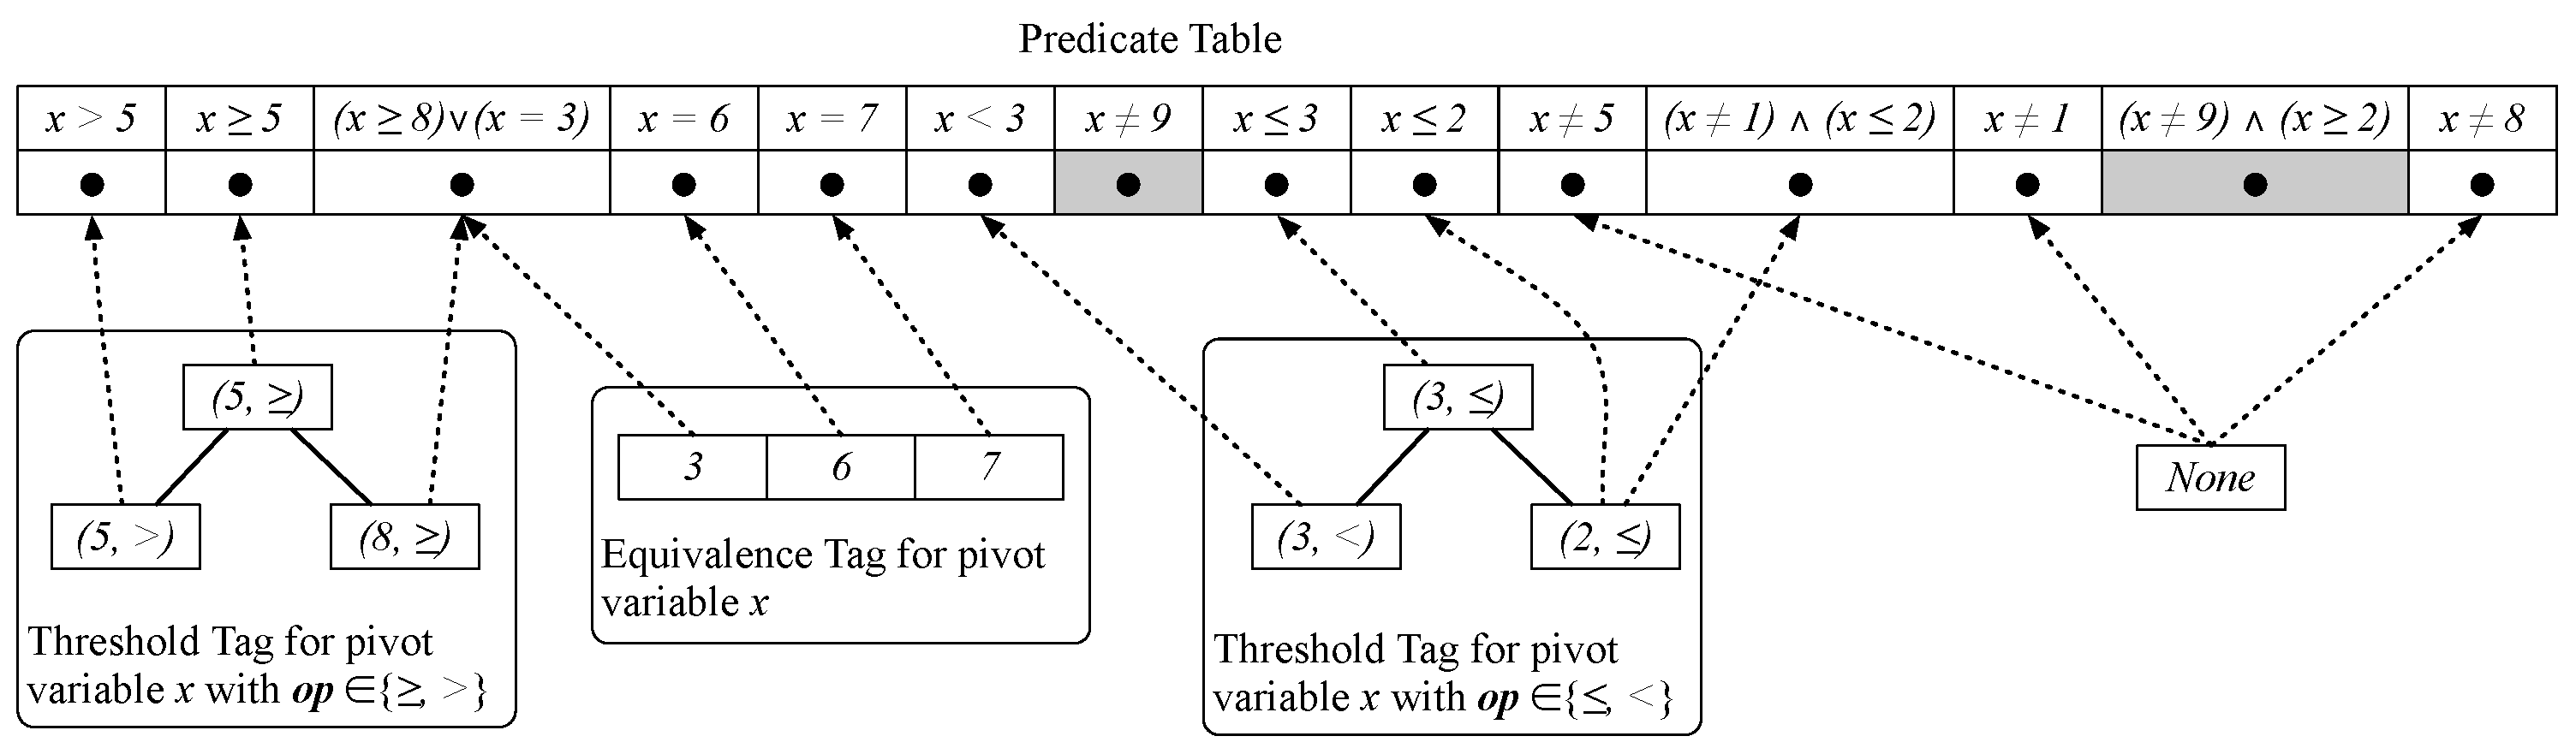
\includegraphics[width=180mm]{fig/manager.eps}
  \caption{A example of the condition manager in AutoSynch}
  \label{fig:mgr}
\end{figure*}


When a predicate is added to the condition manager, the predicate is analyzed
and its tags are created and stored in an appropriate data structure. 
Fig.~\ref{fig:mgr} shows an example. The symbol $\bullet$ indicates 
a condition variable. The gray blank indicate the predicate is inactive,
that is, no thread waits on it. A hash table is used for
storing equivalence tags with the general expression $x$. In addition, 
a min-heap and a max-heap are used for threshold tags. 

%\begin{definition}
%    A predicate is inactive if there is no thread waiting on it. Otherwise, we
%    say the predicate is active.
%\end{definition}


For finding a predicate that is true in Fig.~\ref{fig:mgr}, the value of $x$ is 
examined. Suppose at this point $x=4$. We check the hash table with a
constant time and cannot find a tag that is true. Then we check the root of 
the max-heap and min-heap. Again, we find that both tags in the roots are
false. Then we search for the predicates with the $None$ tag exhaustively. We 
find $x \ne 5$ and signal the corresponding condition variable. As can
be expected, the equivalence and threshold tags is helpful for searching a 
predicate that is true.   


A predicate must be removed from the tag once no thread waits on 
it to avoid unnecessary predicate evaluation. A threshold tag also needs to be
removed once it has no predicate. The reason is that 
we signal the root of the threshold predicate, an empty root 
will introduce overhead to find the next tag. 

Predicates may be reused. Instead  of removing those predicate with no waiting
thread, 
we move those predicate to an inactivate list. If they are used later, then we 
put them back. Otherwise, when the length of inactivate list exceeds some 
threshold, we remove the oldest predicates from the list.
%\clearpage


\section{Evaluations} \label{sec:eval}
%\subsection{Saturation}
\subsection{Environment}
All of the experiments were conducted on a machine with 16 
Intel(R) Xeon(R) X5560 CPUs and 64 GBs memory. 
%Four kinds of experiments were performed to evaluate the performances of the
%explicit-signal monitor with original Java and the automatic-signal monitor with
%AutoSynch framework. 


\subsection{Signaling mechanisms}
Four implementations using different signaling mechanisms have been 
compared. 
\begin{description}
    \item[Explicit-signal] Using the original Java explicit-signal mechanism. 
    \item[AutoSynch] Using the approach described in this paper. 
    \item[AutoSynch-T] Using the approach described in this paper but excluding
        predicate tagging. 
    \item[Baseline] Using the automatic-signal mechanism relying on only
        one condition variable. It calls $signalAll$ all the time to check the
        predicates.
\end{description}

\subsection{Test problems}
\begin{description}
    \item[Producer-Consumer (PC)] The traditional producer-consumer shown in 
        Fig.~\ref{fig:bb_exp}.
    \item[Producer-Consumer* (PC*)] The producer-consumer* problem shown in
        Fig.~\ref{fig:sigAll_exp}. 
    \item[Round-Robin Access Pattern (RR)] Every test thread accesses the
        monitor in round-robin order. 
    \item[Readers/Writers (RW)\cite{chp71}] The first approach is not FIFO
        \cite{bh75b}. In the approach \cite{bh05}, a ticket is used
        to maintain the accessing order of readers and writers. Every reader
        and writer get a ticket number indicating its arrival order. Readers
        and writers are waiting on the monitor for their turn. Our experiments
        are based on this approach. 
\end{description}

Tab.~\ref{tab:complexity} summarizes the computing complexity for maintaining 
condition variable and deciding which thread should be signaled. The column $C$
indicates the computing complexity for maintaining condition variable, while 
the column $S$ indicates the computing complexity for deciding which condition 
variable should be signaled. Note that, for producer-consumer* problem, it
takes $O(ln(n))$ to maintain the condition variable in $AutoSync$. The reason 
is that we use heap as underlying data structure for threshold predicates. The 
computing complexity of add and remove operations is $O(ln(n))$.

\begin{table*}[ht!]
   \centering
   \begin{tabular}{|c||c|c||c|c||c|c||c|c|}
      \hline 
      & \multicolumn{2}{c||}{PC} & \multicolumn{2}{c||}{PC*} & 
        \multicolumn{2}{c||}{RR} & \multicolumn{2}{c|}{RW} \\
      \hline
         & C & S & C & S & C & S & C & S \\
      \hline 
      \hline 
      explicit & $O(1)$ & $O(1)$ & $O(1)$ & $O(n^2)$ & $O(1)$ & $O(1)$ & $O(1)$ &
      $O(1)$ \\
      \hline 
      baseline & $O(1)$ & $O(n^2)$ & $O(1)$ & $O(n^2)$ & $O(1)$ & $O(n^2)$ &
      $O(1)$ & $O(n^2)$ \\
      \hline 
      AutoSynch-T & $O(1)$ & $O(1)$ & $O(1)$ & $O(n)$ & $O(1)$ & $O(n)$ & $O(1)$ 
      & $O(n)$ \\
      \hline 
      AutoSynch & $O(1)$ & $O(1)$ & $O(ln(n))$ & $O(1)$ & $O(1)$ & $O(1)$ & 
      $O(1)$ & $O(1)$\\
      \hline 
   \end{tabular}
   \caption{The computing complexity}
   \label{tab:complexity}
\end{table*}

\begin{table*}[ht!]
   \centering
   \begin{tabular}{|c||c|c||c|c||c|c||c|c|c|c|c|}
      \hline 
      & \multicolumn{2}{c||}{await} & \multicolumn{2}{c||}{lock} & 
        \multicolumn{2}{c||}{signalOne} & \multicolumn{2}{c|}{Tag Mger} &
        \multicolumn{2}{c|}{others} & total \\
      \hline
         & T & \% & T & \% & T & \% & T & \% & T & \% & T \\
      \hline 
      \hline 
      explicit & $21365$ & $99.7\%$ & $28$ & $0.15\%$ & $NA$ & $NA$ & $NA$ &
      $NA$  & $28$ & $0.15\%$ & $21433$ \\
      \hline 
      AutoSynch-T & $410377$ & $98.5\%$ & $3140$ & $0.7\%$ & $2108$ & $0.5\%$
      & $NA$ & $NA$ & $1033$ & $0.2\%$ & $416658$\\
      \hline 
      AutoSynch & $96754$ & $98.8\%$ & $812$ & $0.8\%$ & $112$ & $0.1\%$ & 
      $124$ & $0.1\%$ & $148$ & $0.02\%$ & $21433$\\
      \hline 
   \end{tabular}
   \caption{The CPU usage for round robin}
   \label{tab:cpu}
\end{table*}


%\subsection{Testbed}
%Fig.~\ref{fig:testbed} shows the experimental testbed \cite{bfc95}. 
%Every test thread has two state, monitor state and workload state. A thread
%query to access monitor in monitor state and perform its own job on workload
%state. The average response time of the monitor allows us evaluate the
%performance of different monitors. The first part of the experiments assume
%no workload for every thread. That is, every thread executes only monitor
%accessing calls with no other work. In the second part, we compared the
%performance under different workload.  
%\begin{figure}[ht!]
%  \centering
%  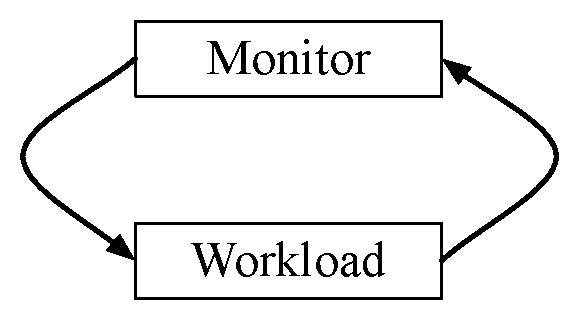
\includegraphics[width=40mm]{fig/testbed.eps}
%  \caption{The testbed}
%  \label{fig:testbed}
%\end{figure}
%
%\subsection{Saturation evaluation}
\subsection{Experimental results}


Fig.~\ref{fig:pc_eval} shows the results of producer-consumer problem. The 
x-axis indicates the number of producers and consumers; the y-axis indicates 
the runtime in milliseconds. Total 
512000 $put$ and $take$ operations were executed by
all producers and consumers. As expected, the baseline is much slower than
other three signaling mechanisms, which have similar performance. This 
phenomenon can be explained as follows. There are only two waituntil statements 
with global predicates, $count > 0$ and $count < items.length$. Therefore, the 
complexity for signaling a thread in AutoSynch and AutoSynch-T are also constant. 
Hence, both AutoSynch and AutoSynch-T are as efficient as explicit-signal 
mechanism. 

\begin{figure}[ht!]
  \centering
  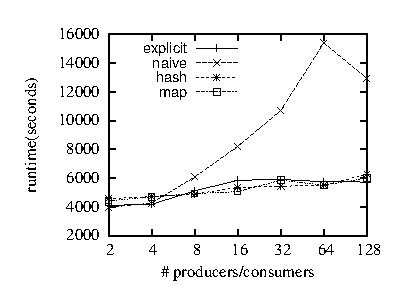
\includegraphics[width=80mm]{fig/pc.eps}
  \caption{The results of producer-consumer problem}
  \label{fig:pc_eval}
\end{figure}

Fig.~\ref{fig:rpc_eval} shows the results of producer-consumer* problem. Total
512000 items are $put$ and then $taken$. The x-axis indicates the number of 
consumers; the y-axis indicates the runtime in milliseconds. Only one producer
was in this experiment. The producer put a item into the buffer a time. A 
consumer randomly take $b/2$ ~ $b$ items a time, where $b = 128$ is the size of 
the buffer. Fig.~\ref{fig:rpc_eval} indicates that AutoSynch and AutoSynch-T are
much faster than the baseline and the explicit-signal mechanism. The reason is
that both explicit-signal mechanism and baseline use signallAll calls. In this
experiment setup, many unnecessary context switches were introduced since a
consumer takes a large amount of items a time but the producer only puts one
item a time. Both AutoSynch and AutoSynch-T are similar in
Fig.~\ref{fig:rpc_eval} due to the scaling. We compare them in
Fig.~\ref{fig:rpch_eval}. As can be seen, the AutoSynch has a consistent
performance even when the number of producers increases. Although AutoSynch-T has
slightly better performance when the number of producers is small; its 
performance decrease significantly as the number of producers increases. It can
be explained as follows. AutoSynch has some computing overhead in maintaining 
tags and predicates. When the number of producers is small, the benefit of
predicate tagging is less than the computing overhead. However, AutoSynch is
much more scalable with this slight performance sacrifice.

\begin{figure}[ht!]
  \centering
  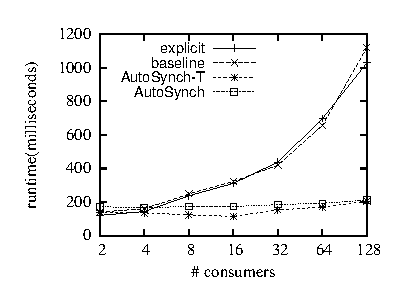
\includegraphics[width=80mm]{fig/rpc.eps}
  \caption{The results of producer-consumer* problem}
  \label{fig:rpc_eval}
\end{figure}

\begin{figure}[ht!]
  \centering
  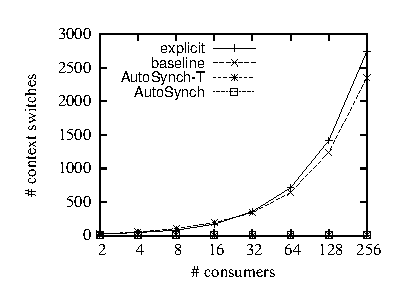
\includegraphics[width=80mm]{fig/csrpc.eps}
  \caption{The number of context switches of producer-consumer* problem}
  \label{fig:csrpc_eval}
\end{figure}

\begin{figure}[ht!]
  \centering
  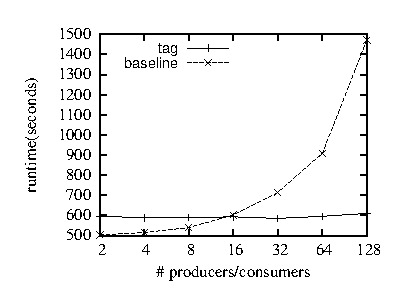
\includegraphics[width=80mm]{fig/rpch.eps}
  \caption{The results of producer-consumer* problem comparing AutoSynch and
  AutoSynch-T}
  \label{fig:rpch_eval}
\end{figure}

%Fig.~\ref{fig:rw_eval} shows the results of reader-writer problem. The
%x-axis indicates the number of readers and writers; the y-axis indicates the
%runtime in seconds. Total 1280 read/write operations were executed by all
%readers and writers. Since readers can read with each other at the same time.
%The runtime decreases as number of readers increases. Need to figure out why 
%explicit-signal approach is so slow in 1/5. Maybe the implementation? 
%


%The dining philosophers problem is often used in computer science to describe 
%the synchronization issues. There are N philosophers siting around at a table 
%with a dish in front of them and a chopstick in between each philosopher. A 
%philosopher only think or eat. A philosopher needs to pick two chopsticks at the
%same time for eating and he does not put down a chopstick until he finishes 
%eating. If the chopstick is hold by another philosopher, then the philosopher 
%who want to eat must wait. In addition, a philosopher cannot eat forever, which
%means he will put down chopstick eventually. Every philosopher must be able to
%eat eventually if he is hungry. Figure 3. illustrate the experimental results
%of the dining philosophers problem. The x-axis depicts the runtime and the 
%y-axis describes the number of philosophers. As can be seen, three approaches 
%has the similar results. The implementations of Naive and N-condition are as 
%efficient as the implementation of explicit signal monitor. 
%
Fig.~\ref{fig:rr_eval} shows the results of round-robin access pattern. The
x-axis indicates the number of threads; the y-axis indicates the
runtime in milliseconds. In this set of experiments, threads are allowed to enter a
monitor in round-robin scheduling. Total 128000 operations were performed on 
the monitor. In this set of experiment, the explicit-signal mechanism has an 
advantage since it can explicitly signal the next thread to enter the 
monitor. Since the baseline is around 50 times slower than the explicit-signal
mechanism, the result of baseline is not plotted in Fig.~\ref{fig:rr_eval} due
to the scaling issues. 
As can be seen, the performance of explicit-signal mechanism is steady 
as the number of thread increases. In comparison with AutoSynch-T, the runtime 
increases significantly as the number of thread increase. For AutoSynch, the 
performance is slower than the explicit-signal mechanism between 2.3 to 2.4
times. However, the performance of AutoSynch does not decrease as the number of
threads increases. 

\begin{figure}[ht!]
  \centering
  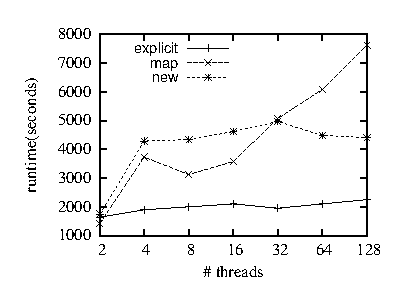
\includegraphics[width=80mm]{fig/rr.eps}
  \caption{The results of round-robin access pattern}
  \label{fig:rr_eval}
\end{figure}


%\subsection{Practical}
%Fig.~\ref{fig:dp_eval} shows the results of dining philosophers problem. The
%x-axis indicates the number of philosophers; the y-axis indicates the
%runtime in seconds. Every philosopher performed 100 eat operations with a
%randomly thinking time between 1 to 20 
%milliseconds. Fig.~\ref{fig:dp_eval} does not show the results of N-Condition 
%implementations since the results are much worse than other implementations. It
%takes around 10 minutes for 128 philosophers. The reason is that many waituntil
%statements with local predicate are used in this problem. Therefore, many
%condition variables are created and removed at runtime. As can be seen, the
%other three approaches have the similar results. This phenomenon can be
%explained as follows. The thinking time is much larger than the synchronization 
%time in the monitor. Therefore, the runtime is dominated by the thinking time.
%%These results suggest that if applications do not have many operations to access
%%a monitor, the performance will not have much difference in automatic-signal and
%%explicit-signal monitor.
%
%
%\begin{figure}[ht!]
%  \centering
%  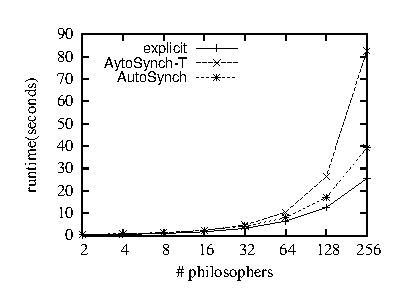
\includegraphics[width=80mm]{fig/dp.eps}
%  \caption{The results of dining philosophers problem}
%  \label{fig:dp_eval}
%\end{figure}

%\begin{figure}
%  \centering
%  \subfloat[Explicit-Signal] {
%    \fbox{
%      \BUseVerbatim[fontsize=\footnotesize]{ExplicitTicketReadersWriters}
%    }
%    \label{subfig:rw_exam_exp}
%  }
%  \\
%  \subfloat[Automatic-Signal] {
%    \fbox{
%      \BUseVerbatim[fontsize=\footnotesize]{AutoSynchTicketReadersWriters}
%    }
%    \label{subfig:rw_exam_imp}
%  }
%  \caption{Random Bounded-buffer example}
%  \label{fig:rbb_exp}
%\end{figure}

%Fig.~\ref{fig:rw_eval} shows the results of reads/writers problem. The
%x-axis indicates the number of writers; the y-axis indicates the
%runtime in milliseconds. In this set of experiments, the number of readers in
%the 5 times of the number of writers. Total 128000 reads and writes were performed on 
%the monitor. The same, the result of baseline is not plotted in Fig.~\ref{fig:rw_eval} due
%to the scaling issue. 
%As can be seen, the performance of explicit-signal mechanism is steady 
%as the number of thread increases. In comparison with AutoSynch-T, the runtime 
%increases significantly as the number of thread increase. For AutoSynch, the 
%performance is slower than the explicit-signal mechanism between 2.3 to 2.4
%times. However, the performance of AutoSynch does not decrease as the number of
%threads increases. 

Fig.~\ref{fig:rw_eval} shows the results of readers/writers problem. The
x-axis indicates the number of writers and readers; the y-axis indicates the
runtime in milliseconds. The ratio of the number of writers to the number of
readers is fixed at 1 to 5 in all cases. Total 128000 write/read operations are
performed by each writer and reader. Note that, multiple readers can perform
their read operations simultaneously; therefore, the performance may increases
as the number of readers increases. In comparison with AutoSynch-T, the
performance of AutoSynch-T is better than AutoSynch when the numbers of writers
and readers are small. The runtime of AutoSynch-T increases significantly as 
the number of thread increases. AutoSynch outperformed AutoSynch-T when the
numbers of writers and readers are greater than 16 and 80 respectively. For 
AutoSynch, the performance is slower than the explicit-signal mechanism between 
1.5 to 1.8 times.


\begin{figure}[ht!]
  \centering
  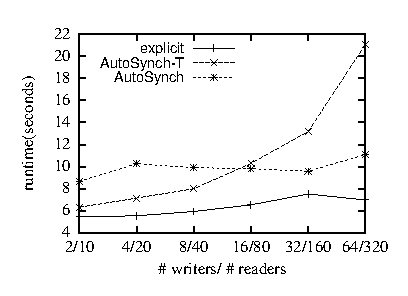
\includegraphics[width=80mm]{fig/trw.eps}
  \caption{The results of readers/writers problem}
  \label{fig:rw_eval}
\end{figure}

%\subsection{Performance under different workload}
%Conduct experiment for readers/writers problem. There is a delay between each
%read/write operation. As the length of delay increase, the workload of the
%monitor decrease. Measure the average response time of the monitor. 

%\begin{figure}[ht!]
%  \centering
%  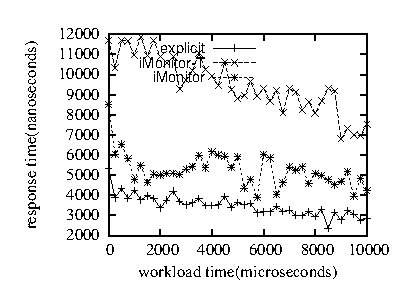
\includegraphics[width=80mm]{fig/strw.eps}
%  \caption{The results of readers/writers problem under different workload}
%  \label{fig:srw_eval}
%\end{figure}

\section{Discussions} \label{sec:dis}
Although the experiment results shows that AutoSynch is 2.33 times slower than 
the explicit-signal mechanism in the worst case, it is still necessary for the 
following reasons: 
\begin{enumerate}
%    \item Potentially gaining performance through optimizing system based on
%        architecture information and avoiding $signalAll$ calls. A $signalAll$ 
%        call introduces unnecessary context switches and decreases performance. 
%        We show that
%        automatic signal monitor can be implemented with almost same efficiency
%        as explicit signals. In fact, in our implementation automatic monitor
%        are sometimes faster than explicit signals. 
    \item Less work for programmers, which implies fewer bugs in programs.
        In explicit-signal monitor, it is the responsibility of programmers to 
        explicitly invoke a $signal$ call on some condition variable for
        conditional synchronization. Using the wrong notification or signaling
        a wrong condition variable are frequent source of bugs. 
    \item Violating separation of concerns. In explicit-signal monitor, the
        conditional synchronization is composed of two parts. A thread checks
        whether or not a condition has met and explicitly waits on a
        condition variable. Another thread detects the condition has met and
        explicit signal the condition variable. The intricate relation between
        threads for conditional synchronization breaks the modularity and 
        encapsulation of programming.  
    \item Mitigating the debugging of explicit-signal programs. It is easier to
        reason a automatic-signal code than a explicit-signal code. A correct
        automatic-signal implementation is helpful in debugging with a 
        explicit-signal implementation. Therefore, $AutoSynch$ can provide  
        rapid prototyping for speedup in developing process and accelerating 
        products time to market.
\end{enumerate}

%fair? FIFO not discussed. performance 


%predicate can include member function?


\section{Conclusion} \label{sec:conclu}
In this paper, we propose AutoSynch framework that supports 
automatic-signal mechanism with $AtuSynch$ class and $waituntil$ statement.
AutoSynch uses the $globalization$ operation to enable the general predicate 
evaluation in every thread. Next, it provides $relay\ guarantee$ that some
thread waiting for a condition has met is always signaled to avoid $signalAll$
calls. AutoSynch also uses predicate tag to accelerate the process in deciding
which thread should be signaled. 

To evaluate the effectiveness of AutoSynch, we built a prototype implementation
using JavaCC \cite{kod04}, Java Compiler Compiler,  and applied it to four
conditional synchronization problems. The experimental results indicate that 
AutoSynch implementations of these problems perform significantly better than
other automatic-signal monitor. Even though AutoSynch is around 2.3 times 
slower than the explicit in the worse case of our experiments, AutoSynch is
around 288 times faster than the explicit-signal in the bounded-buffer* problem 
that relies on $signalAll$ calls. 

In the future, we plan to optimize our framework through using the information 
of architecture. For example, we can get the number of cores of a machine, and
then limit the number of executing threads to avoid unnecessary competition by
using this information. Another area for future work is relaxing the mutual
exclusion when we perform predicate evaluations of $waituntil$ statements. Let
multiple threads can evaluate predicate simultaneously may increase the
performance. 

% use section* for acknowledgement








\appendix
%\section{Bounded-Buffer Code}
%\begin{figure*}[ht!]
%\begin{multicols}{2}
%    \begin{Verbatim}[fontsize=\footnotesize,gobble=8,frame=topline,
%            framesep=5mm,numbers=left,numbersep=2pt,
%            label=\fbox{\small\emph{Explicit-Signal}}]
%        class BoundedBuffer {
%          Object[] items;  
%          int putPtr, takePtr, count;
%          Lock mutex = new ReentrantLock();
%          Condition noSufficientSpace = mutex.newCondition();
%          Condition noSufficientItem = mutex.newCondition();
%          public BoundedBuffer(int n) {
%            items = new Object[n];
%            putPtr = takePtr = count = 0;
%          }
%          public void put(int n) {
%            mutex.lock();
%            while (n + count > items.length) {
%              noSufficientItem.signalAll();
%              noSufficientSpace.await();
%            }
%            for (int i = 0; i < n; ++i) {
%              items[putPtr++] = new Object();
%              if (putPtr == items.length) {
%                putPtr = 0;
%              }
%            }
%            count += n;
%            noSufficientItem.signalAll();
%            mutex.unlock();
%          }
%          public Object[] take(int n) {
%            mutex.lock();
%            while (count < n) {
%              noSufficientSpace.signalAll();
%              noSufficientItem.await();
%            }
%            Object[] ret = new Object[n];
%            for (int i = 0; i < n; ++i) {
%              ret[i] = items[takePtr++];
%              if (takePtr == items.length) {
%                takePtr = 0;
%              }
%            }
%            count -= n;
%            noSufficientSpace.signalAll();
%            mutex.unlock();
%            return ret;
%          }
%        }
%    \end{Verbatim}
%    \begin{Verbatim}[fontsize=\footnotesize,gobble=8,frame=lines,framesep=5mm,
%            numbers=left,numbersep=2pt,
%            label=\fbox{\small\emph{Automatic-Signal}}]
%        monitor class BoundedBuffer { 
%          Object[] items; 
%          int putPtr, takePtr, count; 
%          public void put(int n) { 
%            waituntil(count + n <= items.length); 
%            for (int i = 0; i < n; ++i) {
%              items[putPtr++] = new Object(); 
%              if (putPtr == items.length) { 
%                putPtr = 0; 
%              } 
%            }
%            count += n; 
%          } 
%          public Object[] take(int n) { 
%            waituntil(count >= n);
%            Object[] ret = new Object[n];
%            for (int i = 0; i < n; ++i) {
%              ret[i] = items[takePtr++]; 
%              if (takePtr == items.length) { 
%                takePtr = 0; 
%              }
%            }
%            count -= n;
%            return ret;
%          }
%        }
%    \end{Verbatim}
%\end{multicols}
%  \caption{Bounded-buffer example}
%  \label{fig:npc_exp}
%\end{figure*}
%\section{Readers/Writers Code}
%\begin{figure*}[ht!]
%\begin{multicols}{2}
%    \begin{Verbatim}[fontsize=\footnotesize,gobble=8,frame=topline,
%            framesep=5mm,numbers=left,numbersep=2pt,
%            label=\fbox{\small\emph{Explicit-Signal}}]
%        public class ReadersWritersMonitor {
%          int rcnt;
%          int ticket, serving;
%          Lock mutex = new ReentrantLock();
%          Map<Integer, Condition> mapCondition 
%              = new HashMap<Integer, Condition>();
%          public ReadersWritersMonitor() {
%            rcnt = ticket = serving = 0;
%          }
%          public void startRead() {
%            mutex.lock();
%            int myTicket = ticket;
%            ticket++;
%            Condition cond = mutex.newCondition();
%            mapCondition.put(myTicket, cond);
%            while (myTicket != serving) {
%              if (mapCondition.containsKey(serving)) {
%                 mapCondition.get(serving).signal();
%              }
%              cond.await();
%            }
%            mapCondition.remove(myTicket);
%            rcnt++;
%            serving++;
%            mutex.unlock();
%          }
%          public void endRead() {
%            mutex.lock();
%            rcnt--;
%            mutex.unlock();
%          }
%          public void startWrite() {
%            mutex.lock();
%            int myTicket = ticket;
%            ticket++;
%            Condition cond = mutex.newCondition();
%            mapCondition.put(myTicket, cond);
%            while (myTicket != serving || rcnt != 0) {
%              if (myTicket != serving &&
%                   mapCondition.containsKey(serving)) {
%                 mapCondition.get(serving).signal();
%              }
%              cond.await();
%            }
%            mapCondition.remove(myTicket);
%            mutex.unlock();
%          }
%          public void endWrite() {
%            mutex.lock();
%            serving++;
%            mutex.unlock();
%          }
%        }
%    \end{Verbatim}
%    \begin{Verbatim}[fontsize=\footnotesize,gobble=8,frame=lines,framesep=5mm,
%            numbers=left,numbersep=2pt,
%            label=\fbox{\small\emph{Automatic-Signal}}]
%        public monitor class ReadersWritersMonitor {
%          int rcnt;
%          int ticket, serving;
%          public ReadersWritersMonitor() {
%            rcnt = ticket = serving = 0;
%          }
%          public void startRead() {
%            int myTicket = ticket;
%            ticket++;
%            waituntil(myTicket == serving);
%            rcnt++;
%            serving++;
%          }
%          public void endRead() {
%            rcnt--;
%          }
%          public void startWrite() {
%            int myTicket = ticket;
%            ticket++; 
%            waituntil(myTicket == serving && rcnt == 0);
%          }
%          public void endWrite() {
%            serving++;
%          }
%        }
%    \end{Verbatim}
%\end{multicols}
%  \caption{Readers-writers example}
%  \label{fig:trw_exp}
%\end{figure*}
%\section{Round-Robin Monitor Code}
%\begin{figure}[ht!]
%    \begin{Verbatim}[fontsize=\footnotesize,gobble=8,frame=topline,
%            framesep=5mm,numbers=left,numbersep=2pt,
%            label=\fbox{\small\emph{Explicit-Signal}}]
%        public class RoundRobinMonitor{
%          int numProc;
%          int pid;
%          Lock mutex = new ReentrantLock();
%          Condition[] conds;
%          public RoundRobinMonitor(int n) {
%            numProc = n;
%            pid = 0;
%            Condition = new Condition[n];
%            for (int i = 0; i < n; i++) {
%              conds[i] = mutex.newCondition();
%            }
%          }
%          public void access(int myId) {
%            mutex.lock();
%            while (pid != myId) {
%              conds[pid].signal();
%              conds[myId].await();
%            }
%            pid = (pid + 1) % numProc;
%            conds[pid].signal();
%            mutex.unlock();
%          }
%        }
%    \end{Verbatim}
%    \begin{Verbatim}[fontsize=\footnotesize,gobble=8,frame=lines,framesep=5mm,
%            numbers=left,numbersep=2pt,
%            label=\fbox{\small\emph{Automatic-Signal}}]
%        public monitor class RoundRobinMonitor {
%          int numProc;
%          int pid;
%          public RoundRobinMonitor(int n) {
%            numProc = n;
%            pid = 0;
%          }
%          public void access(int myId) {
%            waituntil(pid == myId);
%            pid = (pid + 1) % numProc;
%          }
%        }
%    \end{Verbatim}
%  \caption{Round-Robin example}
%  \label{fig:rr_exp}
%\end{figure}
%
%
%\acks
%
%Acknowledgments, if needed.
%
%% We recommend abbrvnat bibliography style.
%
%\bibliographystyle{abbrvnat}
%
%% The bibliography should be embedded for final submission.
%
\begin{thebibliography}{}
\softraggedright

\bibitem {bh75a}
  P. Brinch Hansen, \emph{The Programming language concurrent Pascal}. IEEE
  Trans.~Software Engineering, 1(2), 199--207, June, 1975.

\bibitem {bh75b}
    P. Brinch Hansen, \emph{Structured multiprogramming}. Commun.~ACM 15(7),
    574--578, July 1972.

\bibitem {bfc95}
  P. A. Buhr, M. Fortier, and M. H. Coffin, \emph{Monitor Classification}. ACM 
  Computing Surveys, ACM, 27(1), 63--107, 
  Nov. 2005.
  
\bibitem {bh05}
  P. A. Buhr and A. S. Harji, \emph{Implicit-signal monitors}. ACM 
  Transactions on Programming Languages and Systems ACM, 27(6):1270--1343, 
  Nov. 2005.

\bibitem {bute97}
  D. R. Butenhof, \emph{Programming With Posix Threads}.
  Addison-Wesley, MA, 1997.

\bibitem {chp71}
    P. J. Courtois, F. Heymans, D. L. Parnars, \emph{Concurrent control with
    “``readers'' and “``writers''}. Commun.~ACM, 14(10), 667--668, Oct.~1971.

\bibitem{dijk68} 
    E. W. Dijkstra, \emph{The structure of the “``THE''-multiprogramming
    system}. Commun.~ACM, 11(5), 341 -- 346, May 1968. 

\bibitem {gjs00}
    J. Gosling, B. Joy, and G. Steele, \emph{The Java Language Specification}.
    2nd ed. Addison-Wesley, MA, 2000. 

\bibitem {gm05}
    V. K. Garg and N. Mittal, \emph{A Critique of Java for Concurrent
    Programming}, IEEE Distributed Systems online 6(9), 2005.

\bibitem {hwg03}
    A. Hejisberg, S. Wiltamuth, and P. Golde, \emph{C\# Language
    Specification}. Addison-Wesley, MA, 2003.

\bibitem {hoa74}
  C. A. R. Hoare, \emph{Monitors: an operating system structuring concept}. 
  Commun.~ACM, 17(10), 549--557, Oct.~1974. 

\bibitem{kes77} 
    J. L. W. Kessels. \emph{An alternative to event queues for synchronization 
    in monitors}. Commun.~ACM, 20(7), 500--503, July 1977.
  
\bibitem{kod04}
    V. Kodaganallur, \emph{Incorporating language processing into Java 
    applications: a JavaCC tutorial}. IEEE Software, 21(4), 70--77,
    July--Aug.~2004. 

\bibitem{lea05}
    D. Lea, \emph{The java.util.concurrent synchronizer framework}. Science of 
    Computer Programming, 58(3), 293 -- 309, Dec.~2005.

\bibitem{stro97}
    B. Stroustrup, \emph{The C++ Programming Language}. 3rd ed. Addison-Wesley,
    MA, 1997.

\end{thebibliography}
\end{document}
